Um nun Aussagen über die kinetische Energie der Elektronen zu treffen, verwendet man die Gegenfeldmethode. Man löst Elektronen aus einer Photokathode mittels Bestrahlung mit monochromatischem Licht aus. Die ausgelösten Elektronen lässt man gegen eine Gegenspannung $U_{Br}$ anlaufen, die eine bremsende Wirkung auf sie ausübt.\\
Es wird nun eine Gegenspannung auf einen Wert $U_g$ eingestellt, bei dem gerade keine Elektroden mehr an der Kathode ankommen.\\
Damit haben die Elektronen nun die kinetische Energie in potentielle umgewandelt und es gilt
\begin{equation}
\label{eq:Theorie_EnergieGleichung}
h \cdot \nu = U_{g} \cdot e_0 + W_A
\end{equation}
mit der Elementarladung $e_0$.\\

Man kann jedoch auch Abweichungen von dieser Betrachtung feststellen, da die Elektronen nicht allesamt die gleiche Energie besitzen, sondern nach der Fermi-Dirac-Statistik bei Zimmertemperatur eine Energieverteilung besitzen, deshalb kann man nicht den abrupten Abfall des Photostroms beobachten, sondern ein asymptotisch gegen Null strebendes Verhalten, wie in Abb. 1 zu sehen. (vgl. Abbildung 3.1).
\begin{figure}[h]
	\centering
	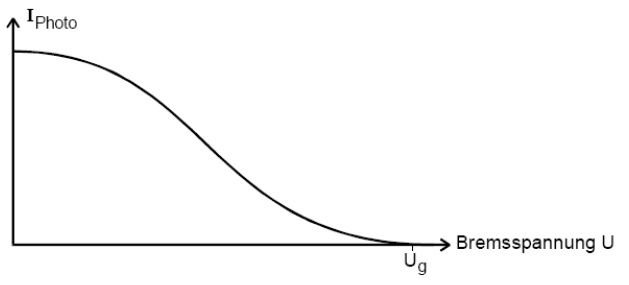
\includegraphics[scale = 0.6,]{Grafiken/V500_Abb1.jpg}
	\caption{Verhalten des Photostroms\cite{V500}}
\end{figure}



\subsection{Aufbau der Photozelle}
Es wird eine sogenannte Photozelle für den eigentlichen Versuch verwendet. Wie Abb. 2 zeigt, besteht die Zelle aus einem evakuierten Glaskolben, in welchem sich die Kathode befindet, die um eine ringförmige Anode angeordnet ist.\\

\begin{figure}[h]
	\centering
	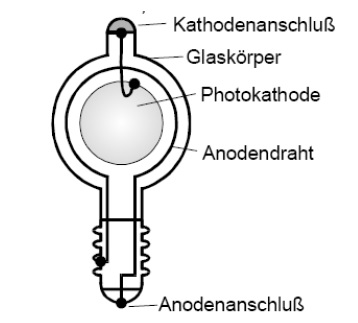
\includegraphics[scale = 0.6, ]{Grafiken/V500_Abb2.jpg}
	\caption{Photozelle\cite{V500}}
\end{figure}
Dabei ist entsprechend die Fläche der Kathode erheblich größer als die der Anode um zu verhindern, dass auch aus der Kathode Photoelektronen austreten. Dies unterdrückt man zusätzlich durch die Verwendung eines Materials das eine erheblich höhere Austrittsarbeit als das Kathodenmaterial besitzt.\\

Dies gilt jedoch nicht uneingeschränkt, denn wenn $A_{Kathode} < h \cdot \nu <  A_{Anode}$ gilt, tritt wegen des viel zu hohen Potentials kein Photostrom auf und die Elektronen können die Anode nicht erreichen. Um diese Potentialbarriere zu überwinden, muss eine beschleunigende Spannung angelegt werden. Dies ist schematisch in Abb. 3 dargestellt.\\

\begin{figure}[h]
	\centering
	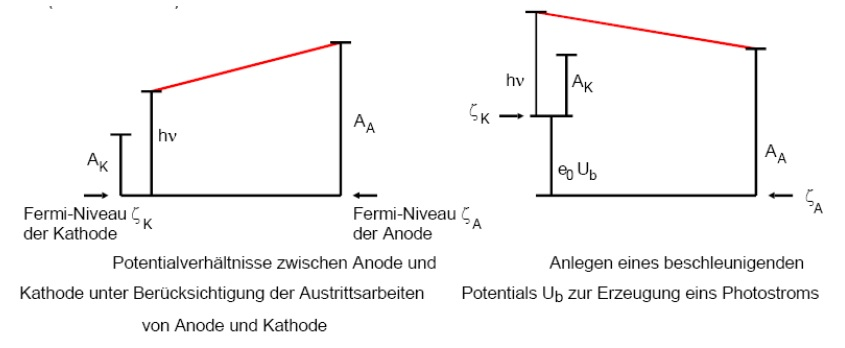
\includegraphics[scale = 0.6,]{Grafiken/V500_Abb3.jpg}
	\caption{Schematische Darstellung der Potentiale an Anode und Kathode\cite{V500}}
\end{figure}

\subsection{Versuchsaufbau}

Um monochromatisches Licht zur Bestrahlung zu erhalten verwendet man Lampen die verschiedene wohlbekannte Spektrallinien emittieren. In diesem Fall sind dies eine Quecksilberdampflampe.\\
Um aus dem Licht monochromatisches Licht zu erhalten, verwendet man den in Abb. 4 dargstellten Aufbau. Man nutzt hierbei den Dispersionseffekt am Glasprisma um die Spektrallinien räumlich voneinander zu trennen. 

\begin{figure}[h]
	\centering
	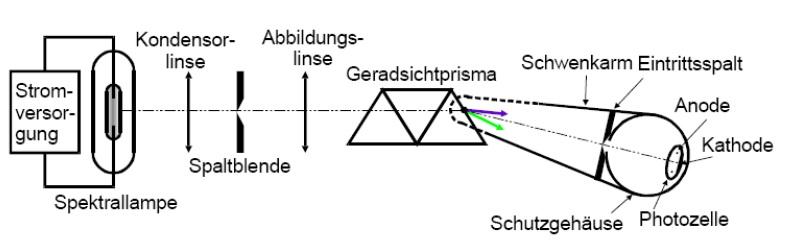
\includegraphics[scale = 0.6,]{Grafiken/V500_Abb4.jpg}
	\caption{optischer Aufbau\cite{V500}}
\end{figure}

Die erste Linse wandelt das Licht in einen parallelen Strahlengang, der nachfolgende Spalt dient der Intensitätsregulierung und die zweite Linse bildet das Licht auf das Glasprisma ab. Diese trennt die Spektrallinien auf um mit monochromatischem Licht die Photozelle beleuchten.\\
Die Linsen sind dabei verschiebbar angeordnet, so dass man sie entsprechend ihrer Brennweite so einjustieren kann, dass man eine scharfe Abbildung der Spektrallinien erhält. 

\begin{figure}[h]
	\centering
	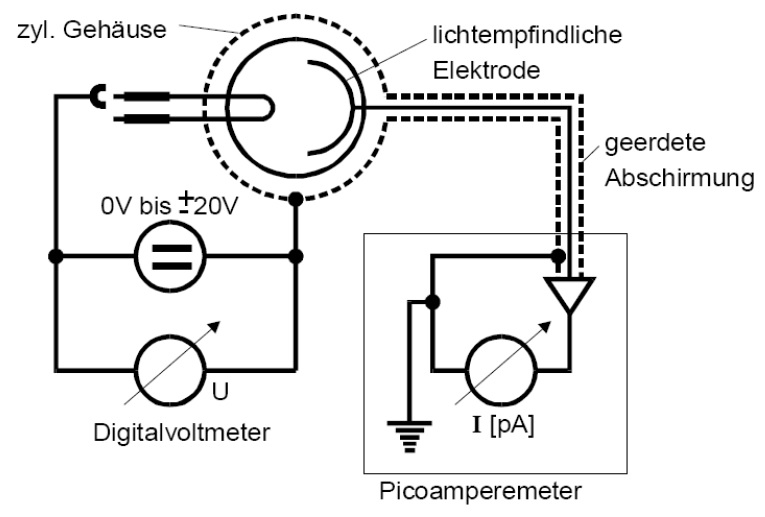
\includegraphics[scale = 0.6,]{Grafiken/V500_Abb5.jpg}
	\caption{Versuchsaufbau\cite{V500}}
\end{figure}

Es wird für die Spektrallinien Gelb, Grün, Blaugrün und zweimal Violett gemessen und anschließend noch einmal für verschiedene Gegenspannungen $U$ von -20 $V$ bis +20 $V$.
